\documentclass[11pt,a4paper]{article} % ein Artikel in 11-Punkt Schrift
% wie man sich schon denkt leitet % einen Kommentar bis Zeilenende ein

\usepackage[german]{babel} % deutsch, deutsche Rechtschreibung
\usepackage[utf8]{inputenc} % Unicode-Zeichensatz bei Textquelle
\usepackage[T1]{fontenc} % Umlaute und deutsches Trennen
\usepackage{mathptmx} % Times New Roman, gewohnter Font
\usepackage{courier} % einen schickeren Schreibmaschinenfont
\usepackage[scaled=.95]{helvet} % was serifenloses, wenn gebraucht
\usepackage{graphicx} % wir wollen Bilder einfügen
\usepackage{xfrac} % schöne Brüche im Fließtext mit sfrac
\usepackage{soul}% für Textauszeichnung (durchstreichen, Farben), vermeiden
\usepackage{amssymb} % für schöne mathematische Symbole
\usepackage[
backend=biber,
style=numeric,
sorting=none
]{biblatex}
\addbibresource{online.bib}



\usepackage{listings} % Schöne Quellcode-Listings [minted wäre besser]
\lstset{basicstyle=\ttfamily, % Schreibmaschinenschrift
  % basicstyle=\sffamily, % etwas schöner 
  columns=[l]flexible, mathescape=true, 
  showstringspaces=false, numbers=left, numberstyle=\tiny}
\lstset{language=python} % und nur schöne Programmiersprachen ;-)
% und eine eigene Umgebung für Listings
\usepackage{float} % eigene Fließobjekte, kommen an beliebigen Stellen vor
\newfloat{listing}{htbp}{scl}
% \newfloat{listing}{htbp}{scl}[section] % Alternativ, numeriere je Abschnitt
\floatname{listing}{Listing} % listing ist ein Fließobjekt

% Auch wenn es anrüchig ist, man kann den Platz etwas mehr ausnützen
\usepackage[paper=a4paper,width=14cm,left=35mm,height=22cm]{geometry}
\usepackage{setspace}
\linespread{1.15} % nicht ganz anderthalbzeilig, nur ein bisschen mehr Platz

%\setlength{\parskip}{0.5em} % kleiner Paragraphen(Absatz)-abstand
%\setlength{\parindent}{0em} % im Deutschen sind Einrückung nicht üblich
\usepackage{parskip} % die Alternative zu den oberen zwei Zeilen
% Übernimmt parksip-Formatierung für den abstract
\usepackage[original]{abstract} 
\setlength{\abstitleskip}{0em} % ansonsten fehlt der erste skip im abstract?

% Seitenmarkierungen 
\usepackage{fancyhdr} % Schickere Header und Footer
\pagestyle{fancy}
% Zeichensatz für Header/Footer
\newcommand{\phv}{\fontfamily{phv}\fontseries{m}\fontsize{9}{11}\selectfont}
\fancyhead[L]{\phv Exposé \\ Bachelor Thesis Cerwenetz} % links oben
\fancyhead[C]{
\includegraphics[width=0.05\textwidth]{hsma_bw}}
\fancyhead[R]{}
\usepackage{url} % wir wollen eine URL anzeigen

% damit wir nicht so viel tippen müssen, nur für Demo
\usepackage{blindtext} 

\begin{document}
%\maketitle % erzeugt den Titel mit Autor und Datum

\section*{Entwicklung eines Frameworks zur Darstellung von Smartphone-Sensordaten
 zur didaktischen Unterstützung von Programmierlehrveranstaltungen} 
\label{sec:intro}
Programmierenlernen birgt für Neueinsteiger Schwierigkeiten.
Abstrakte Konzepte wie Schleifen, Entscheidungsbäume oder Datenstrukturen sind am Anfang nicht leicht zu verstehen.
Die Motivation wird zusätzlich erschwert durch eine beträchtliche Menge an nötiger Vorarbeit um herkömmlich erscheinende Anwendungen zum Beispiel mit einer GUI zu realisieren.
Frameworks wie Swing \cite{swing}, QT \cite{qt} oder Tcl/Tk \cite{tclktk} schaffen hier zwar Abhilfe, benötigen jedoch ebenfalls eine gewisse Einarbeitungszeit.
Alternativ zu herkömmlichen Anwendungen sind simple Embedded Projekte auf Microcontrollern wie zum Beispiel dem Raspberry Pi \cite{raspi}, Microbit\cite{microbit} oder Arduino\cite{arduino} auch ohne graphische Benutzeroberfläche möglich und ermöglichen einen spielerischen Umgang mit dem Programmierernlernen.
\\
Diese Lösungen und Projekte sind unterhaltender und motivierender, erfordern jedoch zusätzliche Microcontroller und gegebenenfalls ergänzende Erweiterungsboards für Sensoren oder Schnittstellen.
Moderne Smartphones sind bereits mit verschiedensten Sensoren ausgestattet, mobiler als Microcontroller und meistens bei Lernenden bereits vorhanden.
\\\\
Im Rahmen der Arbeit soll ein Framework entwickelt werden, was die Sensoren von Smartphones ausliest und Sie angehenden Entwicklerinnen und Entwicklern zur weiteren Verarbeitung zugänglich macht.
Es soll außerdem Aktionen auf dem Smartphone auslösen die gegebenenfalls eine Interaktion mit dem Nutzer ermöglichen.
\\
Das Framework besteht aus drei Teilen: Einer C/C++ Bibliothek, einer in Python implementierten Kontrollanwendung und einer Androidanwendung.
Die Bibliothek stellt Schnittstellen in Form von Objekten und Funktionsaufrufen bereit, die zum Starten von Aktionen auf dem Smartphone dienen.
Außerdem sollen über die Schnittstellen spezifizierte Sensordaten zu festeingestellten Raten automatischen ausgelesen werden.
Umgesetzt werden die Aufrufe auf dem Smartphone durch eine Kontrollanwendung die sich auf dem PC der Entwicklerin bzw. des Entwicklers befindet.
Diese sendet Anweisungen zum Starten von Aktionen an die Anwendung auf dem Smartphone.
In der Smartphoneanwendung werden die Prozeduren ausgeführt und gegebenenfalls Sensordaten an die Kontrollanwendung zurückgesendet.
Die Kontrollanwendung reicht die Sensordaten an die Bibliothek weiter, so dass Sie der Entwicklerin bzw. dem Entwickler zur weiteren Verarbeitung zur Verfügung stehen.
Dieser Vorgang soll über das UDP Protokoll erfolgen, so dass die Bibliothek möglichst wenige Zeilen Code umfasst und schnell in anderen Programmiersprachen wie zum Beispiel Java umgesetzt werden kann.
Die Auswahl an Sensordaten umfassen dabei alle üblichen Smartphone-Sensoren wie zum Beispiel Bewegungs-, Positions oder Umgebungssensoren. 
Eine Übersicht über den Ablauf ist bei Abbildung \ref{fig:Ablauf} zu sehen.
\begin{figure}[htbp]
  \centering
  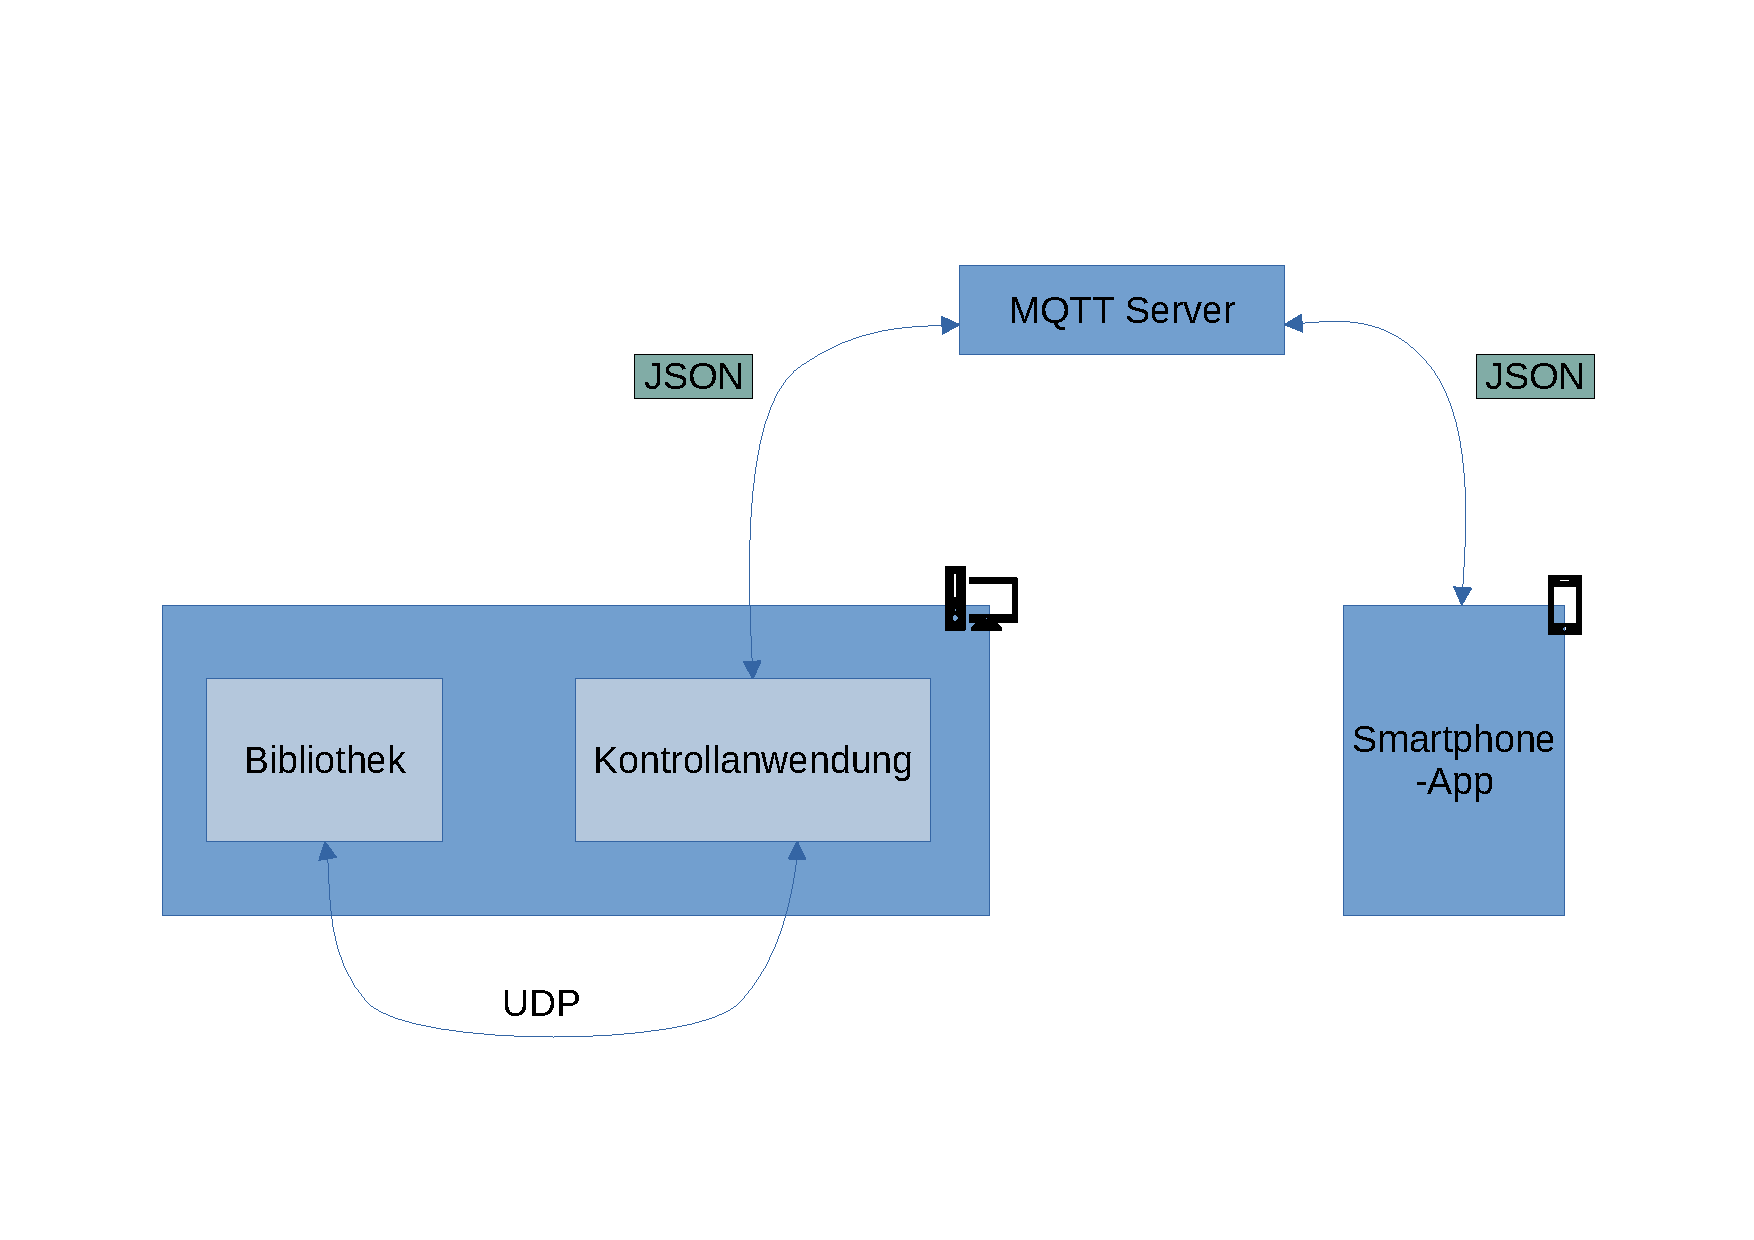
\includegraphics[width=.9\textwidth]{ablauf}
  \caption{Framework-Ablauf}
  \label{fig:Ablauf}
  \end{figure}
\\\\
Zur Vermittlung der beiden Geräte wird zum Nachrichtenaustausch zwischen Kontrollanwendung und Smartphoneanwendung ein MQTT-Server verwendet. \cite{mqtt}
Der Nachrichtenaustausch erfolgt über das JSON-Format \cite{json} für das geeignete Nachrichtenformate definiert werden.
Eine Internetverbindung des PCs und des Smartphones werden somit vorausgesetzt.
Die Konfiguration der korrekten MQTT-Topics auf beiden Geräten wird dabei auf dem PC in einer Konfigurationsdatei und in der Androidanwendung intern über das Shared Preferences-Feature festgelegt.
\\\\
Im Rahmen der Arbeit sollen kleine Demoanwendungsfälle zum Programmierenlernen erarbeitet werden.

\printbibliography
% dann mit "bibtex ausarb" bibtexen und das Literaturverzeichnis ist da
% Besser wäre es mit bibtopic die Quellen sauber zu trennen, siehe thesis

\end{document}
